\section{Circuit Schematics}

The circuits we designed focused on power distribution. Specifically, how were we going to bring the 12V battery supply down to a usable voltage while still supplying enough current for our load? To solve this issue, we designed a voltage regulator using a L7805CV and a DC-DC buck converter using a TPS563200. the buck converter provides a stable 5V to devices like the servo and the Raspberry pi. The buck converter allows us to select a desired output voltage and will supply up to 3A of current to the load.
\begin{figure}[H]
    \centering
    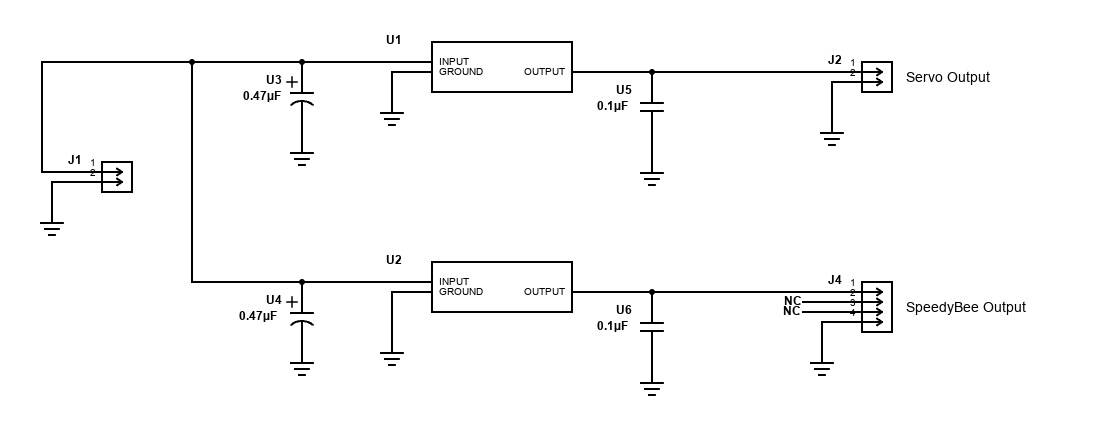
\includegraphics[height=6cm]{Voltage Regulator.png}
     \caption{12V-5V Voltage Regulator}
    \label{fig:Voltage Regulator}
\end{figure}
Fig. \ref{fig:Voltage Regulator} shows the schematic for the voltage regulator used to power both the servo motor and the Raspberry Pi. This circuit is centered around the L7805CV linear voltage regulator, which steps the 12V battery down to a stable 5V output and is capable of supplying up to 1.5A of current. The input and output capacitors are selected based on the recommendations provided in the datasheet to ensure optimal performance in DC applications.
\begin{figure}[H]
    \centering
    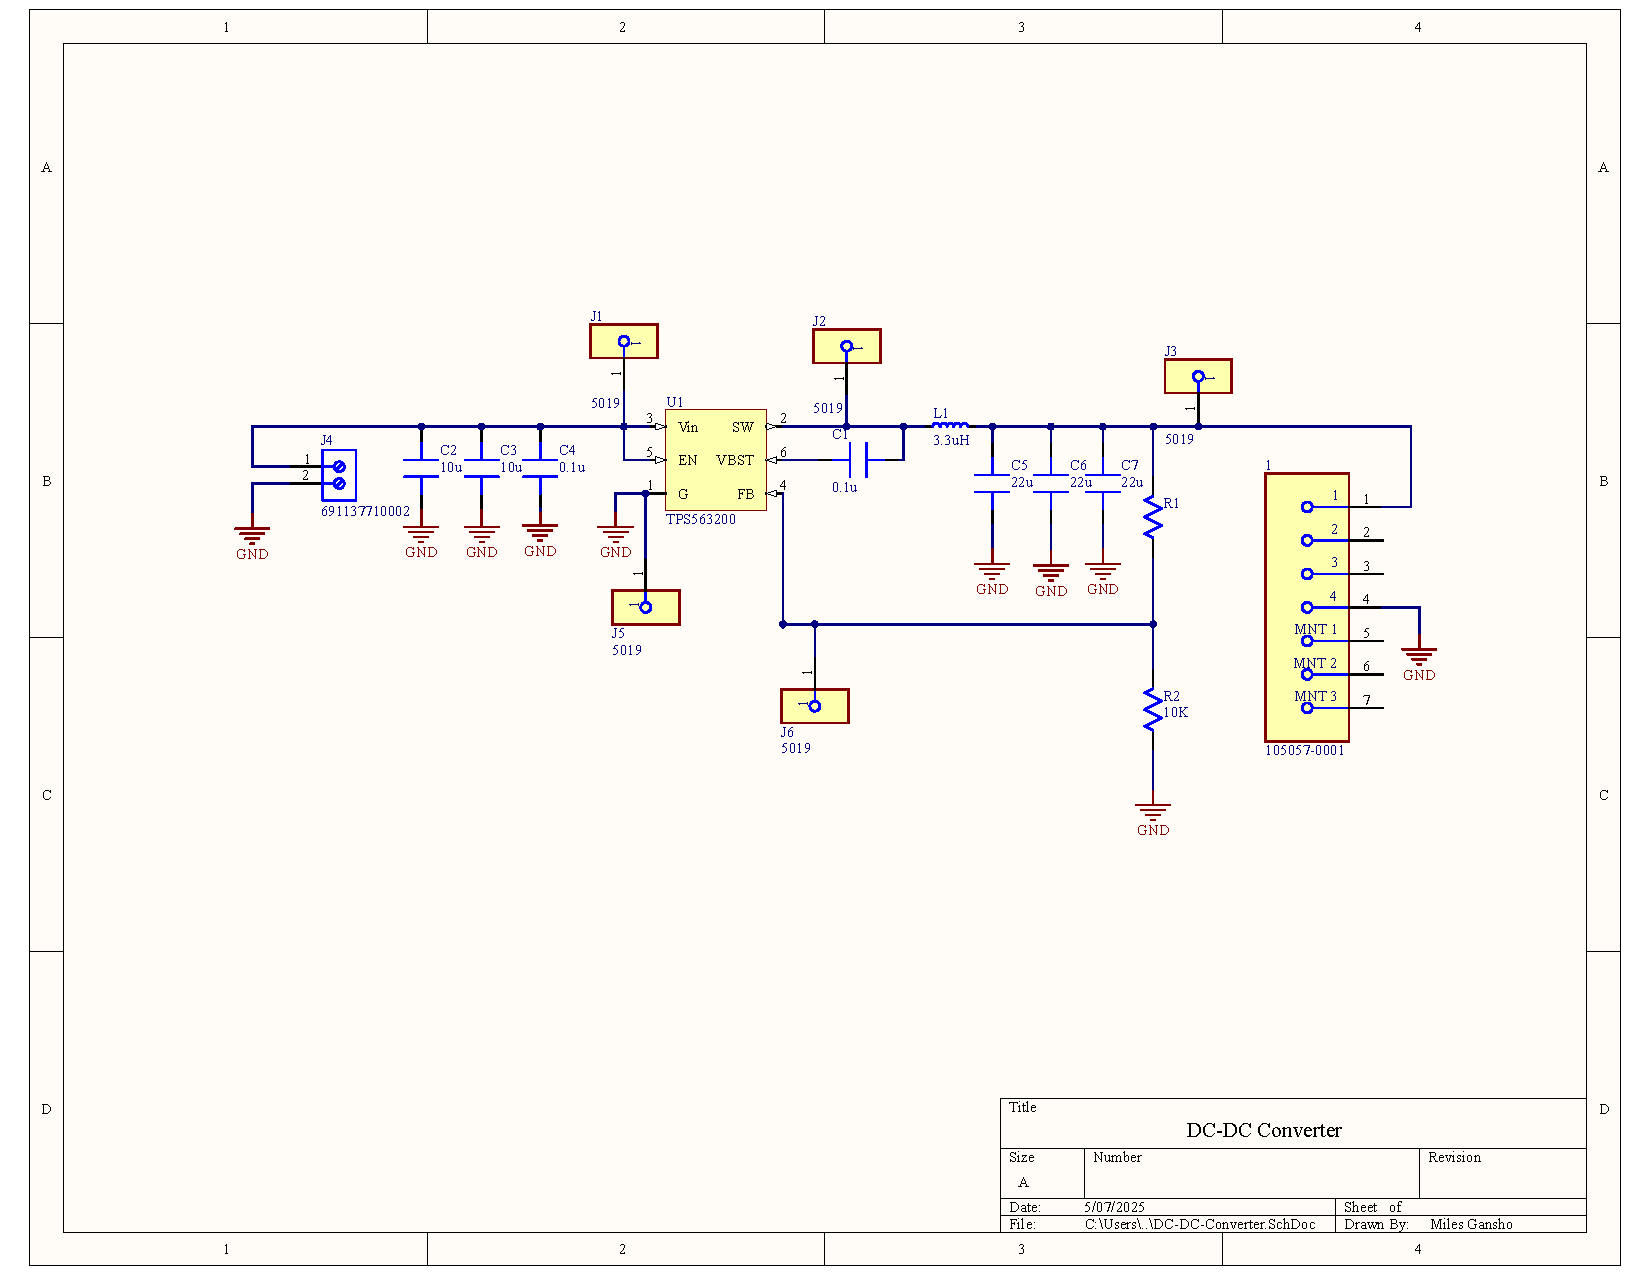
\includegraphics[height=7cm]{DC-DC converter.pdf}
     \caption{DC-DC converter}
    \label{fig:DC-DC Converter}
\end{figure}
Fig. \ref{fig:DC-DC Converter} is the second of our two designed circuits. this circuit also allows us to bring 12V down to a voltage we can use, however the TPS563200 has a feedback on pin 4 which allows us to select a desired output voltage with the voltage divider constructed with R1 and R2. The output capacitors and inductors are selected based on datasheet recommendations for 5-7.5V outputs and R1 is selected using the equation $V_{\text{out}} = 0.765 \times \left(1 + \frac{R_1}{R_2}\right)$. this chip also gives us a output current max of 3A which is much higher then the voltage regulator so better for larger loads.